\chapter{Evaluation}\label{ch:evaluation}
%klare begründung => Anforderung erfüllt ja oder nein


\section{RANSAC Algorithm}

\subsection{Point Clouds: To quantize or not to quantize}\label{subsec:eval-point-clouds}

\subsection{Tests on singular synthetic cube}

A unit cube will be used as a test object to evaluate the RANSAC algorithm.
The cube has been generated with a side length of 1 and a sampling rate of 0.01.
This would equate to a cube with a side length of 1m and a distance of 1cm between points in the real world,
which is comparable to what is provided by the Raw Depth API\@.

\subsubsection{Resilience to Noise}
In figure~\ref{fig:test-noise}, the unit cube is shown with varying noise levels using gaussian noise.
The noise level is defined as the standard deviation of the noise added to the points.


\begin{figure}[ht!]
    \centering
    % First row
    \begin{subfigure}[b]{0.25\textwidth}
        \centering
        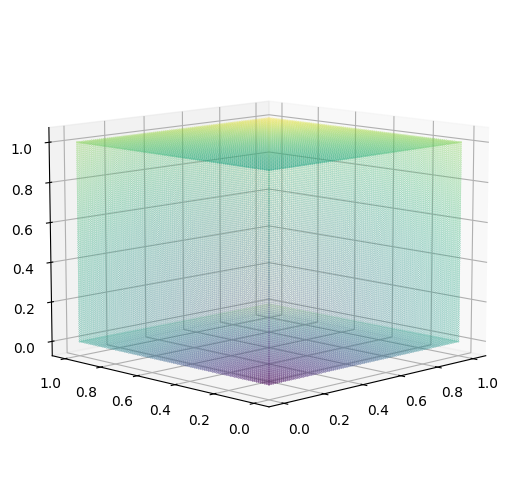
\includegraphics[width=0.9\linewidth]{python/plots/cube_points/data/cube_points_noise_00}
    \end{subfigure}%
    \begin{subfigure}[b]{0.25\textwidth}
        \centering
        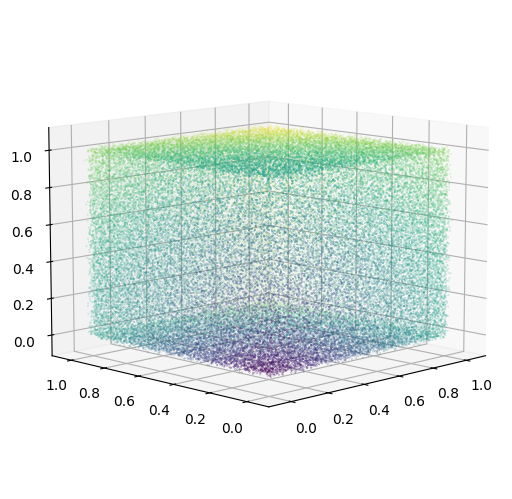
\includegraphics[width=0.9\linewidth]{python/plots/cube_points/data/cube_points_noise_01}
    \end{subfigure}%
    \begin{subfigure}[b]{0.25\textwidth}
        \centering
        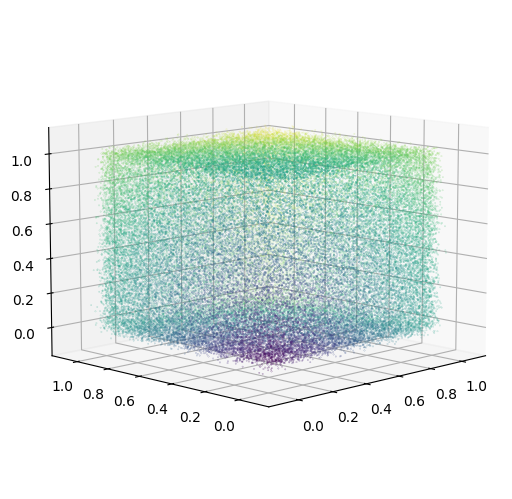
\includegraphics[width=0.9\linewidth]{python/plots/cube_points/data/cube_points_noise_02}
    \end{subfigure}%
    \begin{subfigure}[b]{0.25\textwidth}
        \centering
        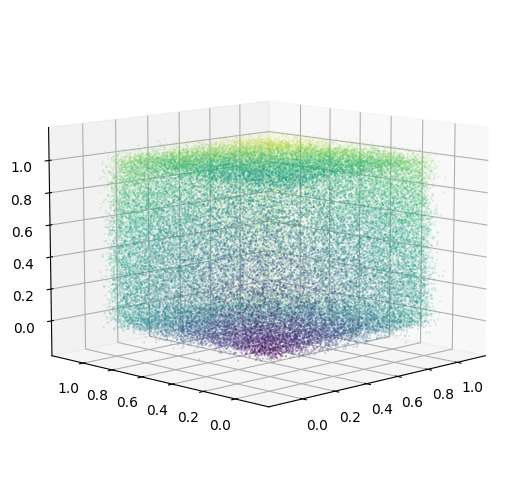
\includegraphics[width=0.9\linewidth]{python/plots/cube_points/data/cube_points_noise_03}
    \end{subfigure}%

%    \vspace{0.5em}

    \begin{subfigure}[b]{0.25\textwidth}
        \centering
        
\includegraphics[width=0.9\linewidth]{python/plots/cube_points/data/cube_points_noise_00_primitives}
        \caption{Noise level 0.00}
    \end{subfigure}%
    \begin{subfigure}[b]{0.25\textwidth}
        \centering
        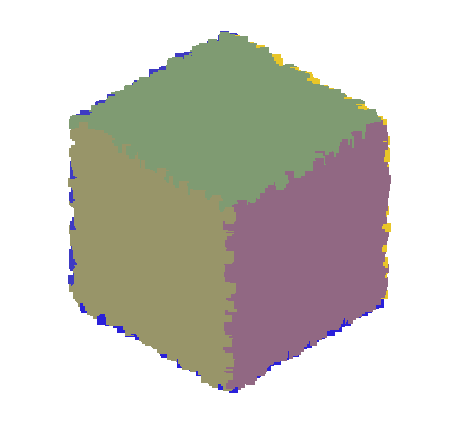
\includegraphics[width=0.9\linewidth]{python/plots/cube_points/data/cube_points_noise_01_primitives}
        \caption{Noise level 0.01}
    \end{subfigure}%
    \begin{subfigure}[b]{0.25\textwidth}
        \centering
        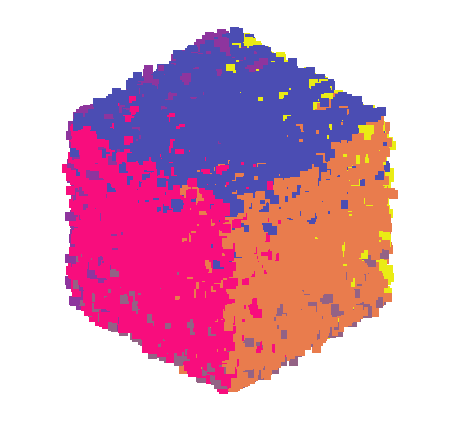
\includegraphics[width=0.9\linewidth]{python/plots/cube_points/data/cube_points_noise_02_primitives}
        \caption{Noise level 0.02}
    \end{subfigure}%
    \begin{subfigure}[b]{0.25\textwidth}
        \centering
        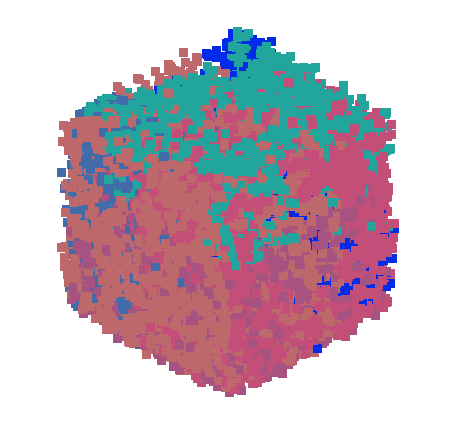
\includegraphics[width=0.9\linewidth]{python/plots/cube_points/data/cube_points_noise_03_primitives}
        \caption{Noise level 0.03}
    \end{subfigure}%

    \caption{Unit cube with varying noise level}
    \label{fig:test-noise}
\end{figure}

\subsubsection{Resilience to missing Data}

As a big problem of depth from motion techniques is the lack of depth information in areas with minimal texture,
the resilience to missing data is crucial.
In figure~\ref{fig:test-missing} points towards the center of the cubes surfaces have been removed.
This mimics the structure of the data of real world data from the Depth API,
as edges are often detected more accurately than surfaces.
To achieve this, points have been removed with an increasing probability based on the
quadratic distance to the center of the face the points belongs to.

%Given a point $x$ with coordinates $(x_1, x_2, x_3)$, edge length $l$, and missing data rate $r$,
%the distance to the closest edge can be calculated as |
%
%As the cube is centered at the origin and aligned with the axis, the absolute of one coordinate will always equal $l/2$.
%By filtering out this coordinate, the point $x$ can be projected onto the plane of the cube,
%resulting in point $x'$ with coordinates $(x'_1, x'_2)$.
%
%The probability $p$ of a point being removed can then be calculated as

%\begin{equation}
%    p = \left(\frac{\sqrt{(l/2 - |x'_1|) \cdot (l/2 - |x'_2|)}}{l / 2}\right)^2 \cdot r
%\end{equation}


\begin{figure}[ht!]
    \centering
    % First row
    \begin{subfigure}[b]{0.25\textwidth}
        \centering
        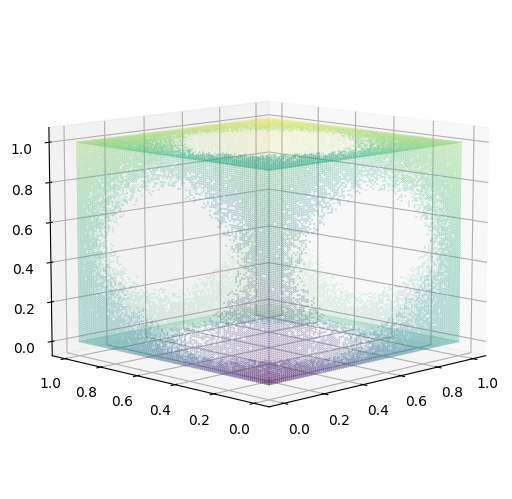
\includegraphics[width=0.9\linewidth]{python/plots/cube_points/data/cube_points_missing_6_0}
    \end{subfigure}%
    \begin{subfigure}[b]{0.25\textwidth}
        \centering
        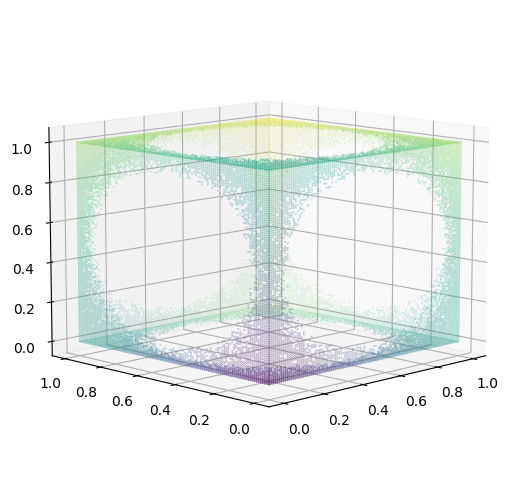
\includegraphics[width=0.9\linewidth]{python/plots/cube_points/data/cube_points_missing_12_0}
    \end{subfigure}%
    \begin{subfigure}[b]{0.25\textwidth}
        \centering
        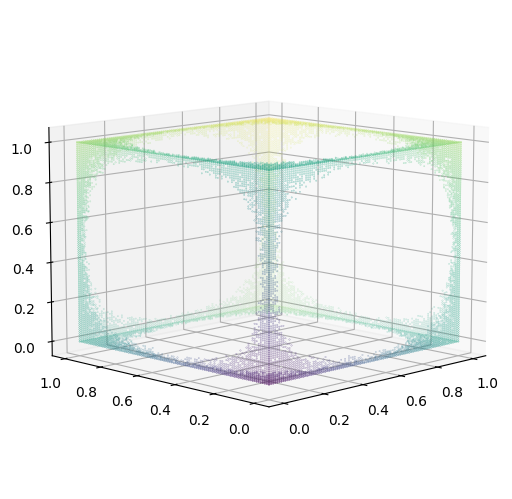
\includegraphics[width=0.9\linewidth]{python/plots/cube_points/data/cube_points_missing_24_0}
    \end{subfigure}%
    \begin{subfigure}[b]{0.25\textwidth}
        \centering
        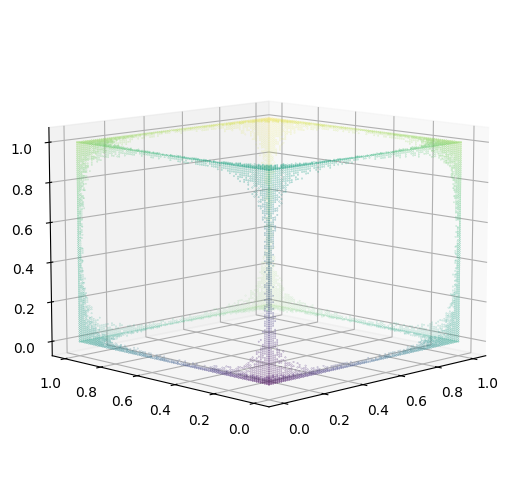
\includegraphics[width=0.9\linewidth]{python/plots/cube_points/data/cube_points_missing_48_0}
    \end{subfigure}%

%    \vspace{0.5em}

    \begin{subfigure}[b]{0.25\textwidth}
        \centering
        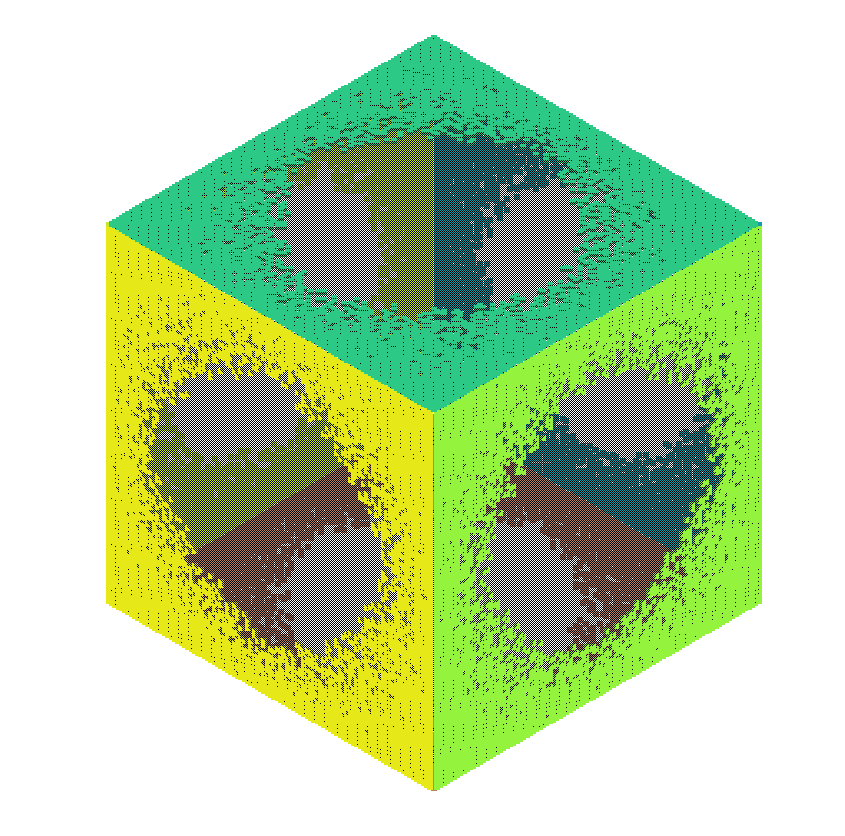
\includegraphics[width=0.9\linewidth]{python/plots/cube_points/data/cube_points_missing_6_0_primitives}
        \caption{Missing level 6}
    \end{subfigure}%
    \begin{subfigure}[b]{0.25\textwidth}
        \centering
        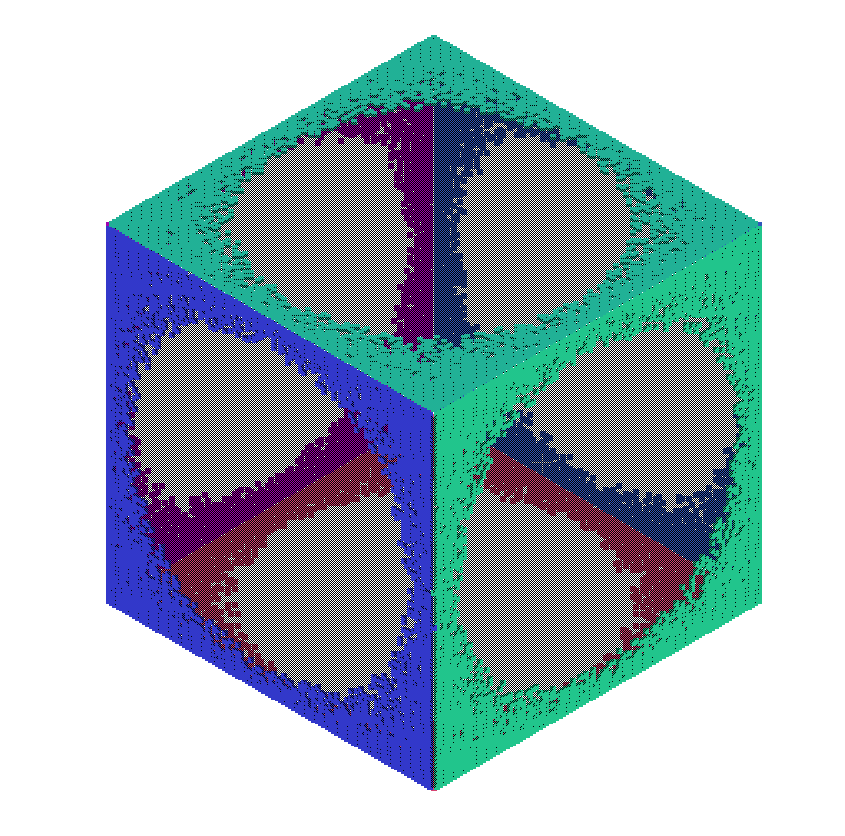
\includegraphics[width=0.9\linewidth]{python/plots/cube_points/data/cube_points_missing_12_0_primitives}
        \caption{Missing level 12}
    \end{subfigure}%
    \begin{subfigure}[b]{0.25\textwidth}
        \centering
        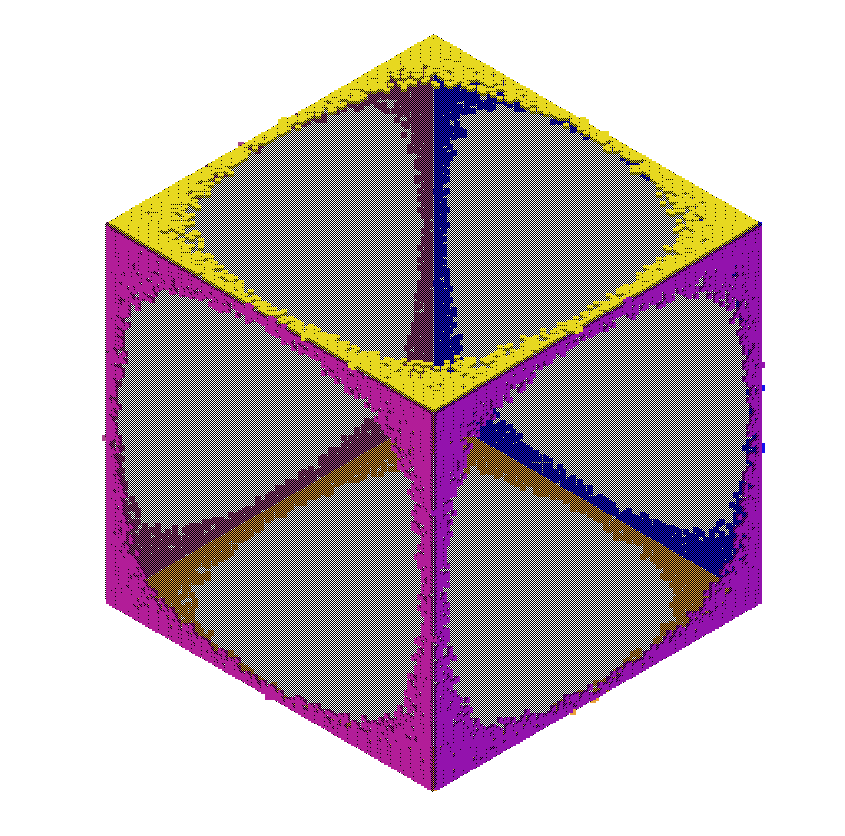
\includegraphics[width=0.9\linewidth]{python/plots/cube_points/data/cube_points_missing_24_0_primitives}
        \caption{Missing level 24}
    \end{subfigure}%
    \begin{subfigure}[b]{0.25\textwidth}
        \centering
        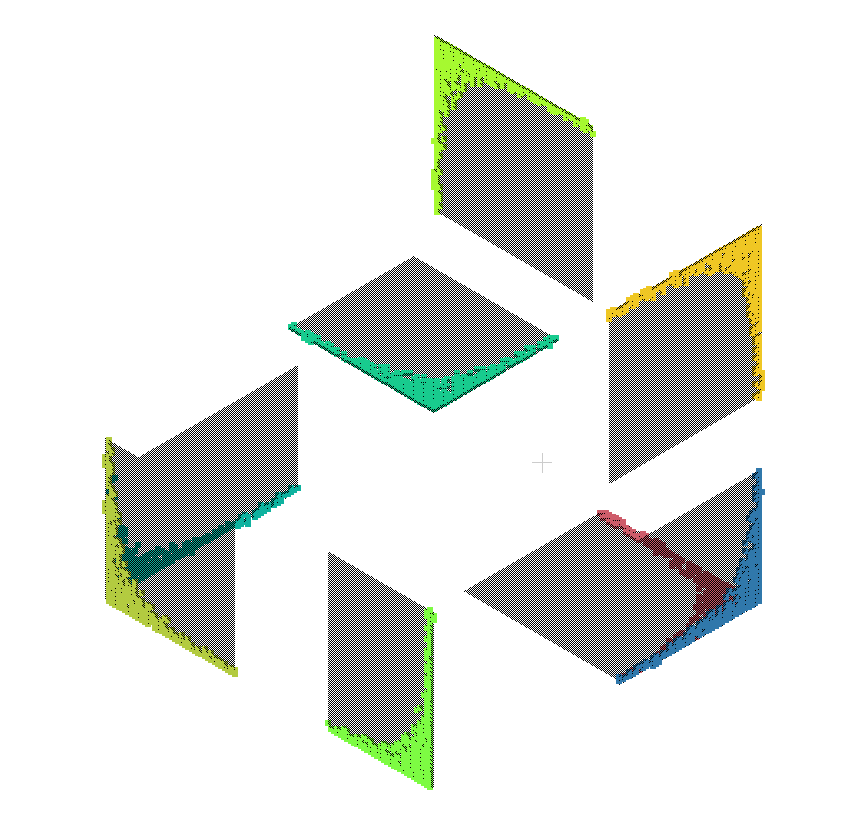
\includegraphics[width=0.9\linewidth]{python/plots/cube_points/data/cube_points_missing_48_0_primitives}
        \caption{Missing level 48}
    \end{subfigure}%

    \caption{Unit cube with varying missing level}
    \label{fig:test-missing}
\end{figure}
